\chapter{Struttura di un file \texttt{.mp3}} \label{chap:struttura_file_mp3}
	
	\mylettrine{P}{rima} di andare ad analizzare come funziona la codifica (e decodifica) MP3, studiamo com'è fatto un file \texttt{.mp3}, ovvero cosa ci si aspetta di ottenere dalla codifica.\\
	\\
	Un file \texttt{.mp3} è suddiviso in parti dette \textit{frame}. Ogni frame contiene 1152 campioni e dura circa 26 \textit{ms}, il che significa che verranno riprodotte circa 38 \textit{fps} (\textit{frame per secondo}). Inoltre, ogni frame è suddiviso in due \textit{granuli} di 576 sample l'uno.\\
	La dimensione in \textit{byte} di ogni frame dipende sia dal bit rate che dalla sampling frequency scelti, secondo la seguente formula:
	
	\begin{equation} \label{eqn:dimensione_frame}
		\mbox{dimensione frame}=\frac{144\cdot\mbox{bitRate}}{\mbox{samplingRate}}+\mbox{padding}.
	\end{equation}
	
	Il bit di \textit{padding} (allocato all'inizio di ogni frame) è utilizzato per rispettare l'esatto bitrate per tutti i frame (dato che dividendo il bitrate per il numero di frame per secondo si potrebbe non ottenere un intero). Se è impostato ad uno allora la dimensione del frame corrispondente viene aumentata di un byte.\\
	Si tenga ben presente che la dimensione di ogni frame dev'essere sempre un intero, in caso contrario si effettuerà un arrotondamento.
	
	\section{Struttura dei frame} \label{sec:struttura_frame}
		
		La struttura generale di ogni frame è mostrata in Figura \ref{fig:frame_layout}.
		
		\begin{figure}[h!]
			\centering
				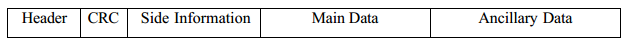
\includegraphics[scale=1]{frame_layout.png}
			\caption{Struttura di un frame.}
			\label{fig:frame_layout}
		\end{figure}
		
		Come possiamo vedere, ogni frame è suddiviso in:
		
		\begin{itemize}
			\item \textit{Header}: detto anche \textit{Intestazione}, è la parte iniziale di ogni frame;
			\item \textit{CRC}: \textit{Cyclic Redundancy Check}, controlla che non ci siano errori nel frame;
			\item \textit{Side Information}: informazione necessaria per decodificare la parte audio del frame;
			\item \textit{Main Data}: gli effettivi dati audio da decodificare;
			\item \textit{Ancillary Data}: detto anche \textit{Dati Ausiliari}, sono dati opzionali destinati a funzioni accessorie.
		\end{itemize}
		
		\subsection{Header} \label{subsec:header}
		
			L'header del frame MP3 ha una lunghezza fissa di 32 bit. La Figura \ref{fig:header_layout} mostra la struttura di un generico frame header.\\
			
			\begin{figure}[h!]
				\centering
					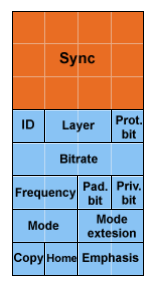
\includegraphics[scale=1.5]{header_layout.png}
				\caption{Struttura dell'header del frame.}
				\label{fig:header_layout}
			\end{figure}
		
		Analizziamo di seguito i vari campi che compongono l'header:
		\begin{itemize}
			\item \textit{Sync} (12 bit): questi bit di sincronizzazione sono sempre impostati tutti a 1 e servono a determinare dove inizia un nuovo frame.
			
			\item \textit{ID} (1 bit): specifica la versione MPEG. Se il bit è asserito significa che il frame è stato codificato con MPEG-1, altrimenti con MPEG-2. Alcuni encoder MP3, inoltre, allocano soltanto 11 bit per la parte Sync per poterne utilizzare 2 per l'ID, secondo la Tabella \ref{tab:campo_id}.
			
				\begin{table}[h!]
					\centering
					\begin{tabular}{|c|c|}
						\multicolumn{1}{c}{\textbf{bit}} & \multicolumn{1}{c}{\textbf{Versione MPEG}}\\
						\hline
						00 & MPEG-2.5 (aggiornamento dell'MPEG-2)\\
						\hline
						01 & Riservato\\
						\hline
						10 & MPEG-2\\
						\hline
						11 & MPEG-1\\
						\hline
					\end{tabular}
					\caption{Valori del campo ID a 2 bit.}
					\label{tab:campo_id}
				\end{table}
				
			\item \textit{Layer} (2 bit): come per il campo ID, i 2 bit del campo Layer indicano quale Layer dello standard MPEG si sta utilizzando, secondo la Tabella \ref{tab:campo_layer}.
			
				\begin{table}[h!]
					\centering
					\begin{tabular}{|c|c|}
						\multicolumn{1}{c}{\textbf{bit}} & \multicolumn{1}{c}{\textbf{Layer MPEG}}\\
						\hline
						00 & Riservato\\
						\hline
						01 & Layer III\\
						\hline
						10 & Layer II\\
						\hline
						11 & Layer I\\
						\hline
					\end{tabular}
					\caption{Valori del campo Layer.}
					\label{tab:campo_layer}
				\end{table}
			
			\item \textit{Protection bit} (1 bit): se asserito, allora viene utilizzato il campo CRC per la rilevazione di errori nel frame.
			
			\item \textit{Bitrate} (4 bit): questi quattro bit, assieme ai campi ID e Layer, informano il decoder sul bitrate richiesto, secondo la Tabella \ref{tab:campo_bitrate}. Ovviamente se il file \texttt{.mp3} è codificato con CBR (Constant BitRate), allora tutti i frame avranno lo stesso valore nel campo Bitrate.
			
				\begin{table}[h!]
					\centering
					\begin{tabular}{c|c|c|c|c|c|c|}
						\multirow{2}{*}{\textbf{bit}} & \multicolumn{3}{|c|}{\textbf{MPEG-1}} & \multicolumn{3}{|c|}{\textbf{MPEG-2}}\\
						\cline{2-7}
						& \textbf{Layer I} & \textbf{Layer II} & \textbf{Layer III} & \textbf{Layer I} & \textbf{Layer II} & \textbf{Layer III}\\
						\hline
						0000 & & & & & &\\
						\hline
						0001 & 32 & 32 & 32 & 32 & 32 & 8\\
						\hline
						0010 & 64 & 48 & 40 & 64 & 48 & 16\\
						\hline
						0011 & 96 & 56 & 48 & 96 & 56 & 24\\
						\hline
						0100 & 128 & 64 & 56 & 128 & 64 & 32\\
						\hline
						0101 & 169 & 80 & 64 & 160 & 80 & 64\\
						\hline
						0110 & 192 & 96 & 80 & 192 & 96 & 80\\
						\hline
						0111 & 224 & 112 & 96 & 224 & 112 & 56\\
						\hline
						
						1000 & 256 & 128 & 112 & 256 & 128 & 64\\
						\hline
						1001 & 288 & 160 & {\color{red} 128} & 288 & 160 & {\color{red} 128}\\
						\hline
						1010 & 320 & 192 & 160 & 320 & 192 & 160\\
						\hline
						1011 & 352 & 224 & 192 & 352 & 224 & 112\\
						\hline
						1100 & 384 & 256 & 224 & 384 & 256 & 128\\
						\hline
						1101 & 416 & 320 & 256 & 416 & 320 & 256\\
						\hline
						1110 & 448 & 384 & 320 & 448 & 384 & 320\\
						\hline
						1111 & & & & & &\\
						\hline
						
					\end{tabular}
					\caption[Valori del campo Bitrate.]{Valori del campo Bitrate (i valori in rosso rappresentano la scelta più frequente).}
					\label{tab:campo_bitrate}
				\end{table}
			
			\item \textit{Frequency} (2 bit): questi 2 bit indicano la sampling frequency utilizzata, come indicato in Tabella \ref{tab:campo_frequency}.
			
				\begin{table}[h!]
					\centering
					\begin{tabular}{|c|c|c|c|}
						\multicolumn{1}{c}{\textbf{bit}} & \multicolumn{1}{c}{\textbf{MPEG-1}} & \multicolumn{1}{c}{\textbf{MPEG-2}} & \multicolumn{1}{c}{\textbf{MPEG-2.5}}\\
						\hline
						00 & 44.1 \textit{kHz} & 22.05 \textit{kHz} & 11.025 \textit{kHz}\\
						\hline
						01 & 48 \textit{kHz} & 24 \textit{kHz} & 12 \textit{kHz}\\
						\hline
						10 & 32 \textit{kHz} & 16 \textit{kHz} & 8 \textit{kHz}\\
						\hline
						11 & \multicolumn{3}{|c|}{Riservato}\\
						\hline
					\end{tabular}
					\caption{Valori del campo Frequency.}
					\label{tab:campo_frequency}
				\end{table}
			
			\item \textit{Padding bit} (1 bit): come già accennato riguardo alla dimensione dei frame, se con la (\ref{eqn:dimensione_frame}) si ottiene un numero decimale, per alcuni frame si arritonderà per eccesso, mentre per altri per difetto. Se ad esempio si utilizza un bitrate di 128 \textit{bps} ed una sampling frequency di 44.1 \textit{kHz}, si avrà la dimensione dei frame pari a circa 417.95 byte, ovvero si avranno frame da 417 e frame da 418, per rispettare il bitrate indicato. Se il bit di padding è settato, allora il frame attuale è stato arrotondato per eccesso.
			
			\item \textit{Private bit} (1 bit): bit a uso specifico delle applicazioni.
			
			\item \textit{Mode} (2 bit): riprendendo quanto detto riguardo alle modalità di canale, i bit Mode indicheranno la modalità del frame attuale secondo la Tabella \ref{tab:campo_mode}.
			
				\begin{table}[h!]
					\centering
					\begin{tabular}{|c|c|}
						\multicolumn{1}{c}{\textbf{bit}} & \multicolumn{1}{c}{\textbf{Channel Mode}}\\
						\hline
						00 & Stereo\\
						\hline
						01 & Joint Stereo\\
						\hline
						10 & Canale Doppio\\
						\hline
						11 & Canale Singolo\\
						\hline
					\end{tabular}
					\caption{Valori del campo Mode.}
					\label{tab:campo_mode}
				\end{table}
			
			\item \textit{Mode Extension} (2 bit): bit utilizzati soltanto nel caso in cui la modalità di canale sia impostata su joint stereo, nel qual caso il campo Mode Extension indicherà se viene utilizzata la tecnica MS stereo, intensity stereo o una combinazione delle due (si veda la Tabella \ref{tab:campo_mode_extension}).
			
				\begin{table}[h!]
					\centering
					\begin{tabular}{|c|c|c|}
						\multicolumn{1}{c}{\textbf{bit}} & \multicolumn{1}{c}{\textbf{MS stereo}} & \multicolumn{1}{c}{\textbf{Intensity stereo}}\\
						\hline
						00 & off & off\\
						\hline
						01 & off & on\\
						\hline
						10 & on & off\\
						\hline
						11 & on & on\\
						\hline
					\end{tabular}
					\caption{Valori del campo Mode Extension.}
					\label{tab:campo_mode_extension}
				\end{table}
			
			\item \textit{Copy} (1 bit): se questo bit è asserito, allora significa che il contenuto è coperto da copyright ed è illegale copiarlo.
			
			\item \textit{Home} (1 bit): se asserito, indica che il frame si trova nel file originale.
			
			\item \textit{Emphasis} (2 bit): bit di enfasi che indicano come ri-equalizzare il suono dopo un'eliminazione del rumore di tipo Dolby (raramente usati). Per conoscenza, si veda la Tabella \ref{tab:campo_emphasis}.
			
				\begin{table}[h!]
					\centering
					\begin{tabular}{|c|c|}
						\multicolumn{1}{c}{\textbf{bit}} & \multicolumn{1}{c}{\textbf{Modello di soppressione del rumore}}\\
						\hline
						00 & Nessuno\\
						\hline
						01 & 50/15 \textit{ms}\\
						\hline
						10 & Riservato\\
						\hline
						11 & CCITT J.17\\
						\hline
					\end{tabular}
					\caption{Valori del campo Emphasis.}
					\label{tab:campo_emphasis}
				\end{table}
			
		\end{itemize}
		
		\subsection{CRC} \label{subsec:crc}
			
			Il campo CRC (di 0 o 16 bit) è una Cyclic Redundancy Check sui dati sensibili del frame, per evitare che contengano errori. Se il bit Protection nell'header è asserito, allora il campo CRC conterrà una checksum dei bit dal 16 al 32 dell'header e della side information (che secondo lo standard contengono i dati più sensibili del frame). Se un frame risulta danneggiato, può essere mutato o rimpiazzato dal frame precedente.
		
		\subsection{Side Information} \label{subsec:side_information}
			
			Il campo Side Information contiene tutte quelle informazioni necessarie al decoder per decodificare i dati audio di ogni frame. Se si utilizza un canale singolo, allora questo campo sarà lungo 17 byte, altrimenti 32. La struttura del campo Side Information è mostrato in Figura \ref{fig:side_information_layout}.\\
			
			\begin{figure}[h!]
				\centering
					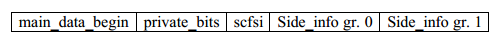
\includegraphics[scale=1.2]{side_information_layout.png}
				\caption{Struttura del campo Side Information.}
				\label{fig:side_information_layout}
			\end{figure}
		
			Analizziamo di seguito i campi della Side Information. Dal momento che le dimensioni dei vari campi possono variare a seconda della modalità di canale scelta, tra parentesi verranno indicate le dimensioni per la modalità mono (primo valore) e le dimensioni per tutte le altre modalità (secondo valore). Se invece è indicato un solo valore, la dimensione di quel campo è costante. Inoltre, tutte le tabelle si riferiscono alla modalità mono.
			
			\begin{itemize}
				\item \textit{main\_data\_begin} (9 bit): utilizzando il formato del Layer III, viene impiegata una tecnica detta \textit{bit reservoir} (letteralmente, \textit{deposito di bit}), che consente di sfruttare lo spazio inutilizzato nel campo Main Data di un frame da frame consecutivi. Il campo main\_data\_begin è un numero negativo che indica quanti byte prima (rispetto al primo bit della synchronization word) iniziano i dati principali, escludendo dal conteggio le parti statiche di un frame, come l'header. Essendo un campo a 9 bit, i dati principali possono iniziare fino a $(2^9-1) \cdot 8 = 4088$ bit prima, che corrisponde a svariati frame. Se il campo è impostato a 0, allora i dati principali iniziano subito dopo la Side Information.
				
				\item \textit{private\_bits} (5 bit, 3 bit): bit privati destinati all'utilizzo specifico da parte delle applicazioni.
				
				\item \textit{scfsi} (4 bit, 8 bit): la \textit{ScaleFactor Selection Information} (o \textit{Informazione sulla Selezione dei Fattori di Scala}) indica se dei certi \textit{scalefactor} (\textit{fattori di scala}, vedremo più avanti cosa sono) sono condivisi oppure no tra i due granuli di un frame. Le bande di fattori di scala sono suddivise in 4 gruppi, secondo la Tabella \ref{tab:gruppi_scalefactor}. In questo campo, vengono trasmessi 4 bit per ogni canale: se il bit del gruppo è asserito, allora quelle scalefactor band valgono sia per il granulo 0 che per il granulo 1, così da poterle trasmettere una sola volta.
				
					\begin{table}[h!]
						\centering
						\begin{tabular}{|c|c|}
							\multicolumn{1}{c}{\textbf{Gruppo}} & \multicolumn{1}{c}{\textbf{Scalefactor Band}}\\
							\hline
							0 & 0, 1, 2, 3, 4, 5\\
							\hline
							1 & 6, 7, 8, 9, 10\\
							\hline
							2 & 11, 12, 13, 14, 15\\
							\hline
							3 & 16, 17, 18, 19, 20\\
							\hline
						\end{tabular}
						\caption{Gruppi delle scalefactor band}
						\label{tab:gruppi_scalefactor}
					\end{table}
				
				\item \textit{Side\_info}: le ultime due parti della Side Information (``Side\_info gr.0'' e ``Side\_info gr.1'') contengono le informazioni per la decodifica dei due granuli del frame e sono strutturalmente identiche (si veda la Figura \ref{fig:side_info_gr_layout}).
				
					\begin{figure}[h!]
						\centering
							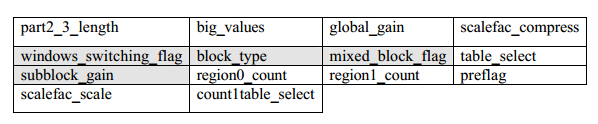
\includegraphics[scale=1]{side_info_gr_layout.png}
						\caption{Struttura della Side Information per ogni granulo.}
						\label{fig:side_info_gr_layout}
					\end{figure}
					
					Di seguito, l'analisi dei sottocampi che compongono la Side Information di ogni granulo:
					
					\begin{itemize}
						
						\item \textit{part2\_3\_length} (12 bit, 24 bit): indica quanti bit allocare nel campo Main Data per i fattori i scala (part2) e per i dati codificati con Huffman (part3) (più avanti vedremo com'è composto il campo Main Data).
						
						\item \textit{big\_values} (9 bit, 18 bit): i 576 sample contenuti in ogni granulo non sono necessariamente codificati tutti con la stessa tabella di Huffman. In particolare, le frequenze di questi sample, che spaziano da 0 al limite di Nyquist, verranno suddivise in 5 regioni (Figura \ref{fig:frequency_regions}), ognuna della quali codificata con una diversa tabella di Huffman. L'obiettivo è quello di rendere la codifica di Huffman ancora più efficiente codificando in modo diverso diverse parti dello spettro.
						
							\begin{figure}[h!]
								\centering
									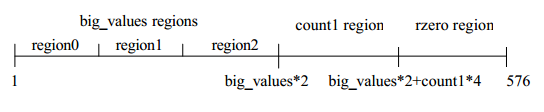
\includegraphics[scale=1]{frequency_regions.png}
								\caption{Regioni di frequenza.}
								\label{fig:frequency_regions}
							\end{figure}
							
							Nella regione rzero si trovano le frequenze più alte, divise a coppie. Nella regione count1 si trovano frequenze più basse di quelle in rzero, suddivise in gruppi di quattro. Infine, nelle regioni big values si trovano tutte le altre frequenze che arrivano fino a zero. Il massimo valore assoluto di ampiezza per i sample nelle regioni big values è limitato a 8191. Dal momento che il campo big\_values determina la grandezza delle regioni big values, il massimo valore possibile per questo campo è 288 \footnote{Calcolato come $576/2$, in quanto la dimensione della regione di big values è calcolata come $big\_values\cdot 2$.}.
						
						\item \textit{global\_gain} (8 bit, 16 bit): specifica la grandezza dello step di quantizzazione.
						
						\item \textit{scalefac\_compress} (4 bit, 8 bit): determina il numero di bit utilizzati per i fattori di scala. Ogni granulo può essere diviso in 12 (per finestre corte) o 21 (per finestre lunghe) bande di fattori di scala. Non spiegheremo qui cosa si intende con finestre, in quanto verrà spiegato più ampiamente all'interno del Capitolo \ref{chap:codifica}. Le bande di fattori di scala sono successivamente suddivise in due parti (0-6, 7-11 per finestre corte e 0-10, 11-20 per finestre lunghe), rispettivamente lunghe \textit{slen1} e \textit{slen2}. A seconda del valore del campo scalefac\_compress, verranno assegnati più o meno bit alle due parti, come mostrato in Tabella \ref{tab:campo_scalefac_compress}.
						
							\begin{table}[h!]
								\centering
								\begin{tabular}{|c|c|c|}
									\multicolumn{1}{c}{\textbf{bit}} & \multicolumn{1}{c}{\textbf{slen1}} & \multicolumn{1}{c}{\textbf{slen2}}\\
									\hline
									0000 & 0 & 0\\
									\hline
									0001 & 0 & 1\\
									\hline
									0010 & 0 & 2\\
									\hline
									0011 & 0 & 3\\
									\hline
									0100 & 3 & 0\\
									\hline
									0101 & 1 & 1\\
									\hline
									0110 & 1 & 2\\
									\hline
									0111 & 1 & 3\\
									\hline
									1000 & 2 & 1\\
									\hline
									1001 & 2 & 2\\
									\hline
									1010 & 2 & 3\\
									\hline
									1011 & 3 & 1\\
									\hline
									1100 & 3 & 2\\
									\hline
									1101 & 3 & 3\\
									\hline
									1110 & 4 & 2\\
									\hline
									1111 & 4 & 3\\
									\hline
								\end{tabular}
								\caption{Valori del campo scalefac\_compress.}
								\label{tab:campo_scalefac_compress}
							\end{table}
						
						\item \textit{windows\_switching\_flag} (1 bit, 2 bit): se asserito, indica che sarà utilizzata una finestra diversa da quella di default (si veda Capitolo \ref{chap:codifica}). Inoltre quando è asserito, tutti i valori (big values) che non sono contenuti nella region0 sono contenuti nella region1, rendendo la region2 di fatto vuota.
						
						\item \textit{block\_type} (2 bit, 4 bit): se il bit windows\_switching\_flag è asserito, allora questo campo serve a indicare il tipo di finestra utilizzato per il granulo corrente. I valori 1 e 3 sono finestre lunghe, mentre il valore 2 indica una finestra corta. Il valore 0 indicherebbe la finestra normale di default (lunga), ma dato che quando si usa la finestra di default il campo block\_type non viene utilizzato, questo valore è vietato. Vediamo nel dettaglio il significato di questi valori in Tabella \ref{tab:campo_block_type} (per i vari tipi di finestra si rimanda sempre al Capitolo \ref{chap:codifica}).
						
							\begin{table}[h!]
								\centering
								\begin{tabular}{|c|c|}
									\multicolumn{1}{c}{\textbf{bit}} & \multicolumn{1}{c}{\textbf{Tipo finestra}}\\
									\hline
									00 & Vietato\\
									\hline
									01 & Finestra inizio\\
									\hline
									10 & 3 finestre corte\\
									\hline
									11 & Finestra fine\\
									\hline
								\end{tabular}
								\caption{Valori del campo block\_type.}
								\label{tab:campo_block_type}
							\end{table}
						
						\item \textit{mixed\_block\_flag} (1 bit, 2 bit): se asserito, indica che le due sottobande più basse (si veda il Capitolo \ref{chap:codifica} per quanto riguarda le sottobande) sono trasformate utilizzando la finestra normale, mentre le restanti 30 utilizzando la finestra indicata dal campo block\_type. Questo campo viene utilizzato soltanto se il bit windows\_switching\_flag è asserito.
						
						\item \textit{table\_select} (10 bit, 20 bit) o (15 bit, 30 bit): lo standard MP3 definisce 32 possibili tabelle di Huffman con cui codificare i sample. Essendo le tabelle possibili 32, servono 5 bit (per canale, granulo e regione) per individuare univocamente una tabella. Il campo table\_select definisce con quali tabelle di Huffman decodificare i sample delle regioni big values. Quindi se windows\_switching\_flag è settato a 1 la regione region2 sarà vuota e si avranno 10 bit (in modalità mono) necessari per l'individuazione delle tabelle di Huffman (20 se in modalità stereo). Se invece il bit è negato si avrà bisogno di altri 5 bit per canale per la tabella relativa alla regione region2, ovvero 15 bit per mono e 30 per stereo.
						
						\item \textit{subblock\_gain} (9 bit, 18 bit): se windows\_switching\_flag=1 e block\_type=10, allora questo campo definisce, 3 bit alla volta, l'offset da aggiungere al global\_gain per ogni sottoblocco.
										
						\item \textit{region0\_count}(4 bit, 8 bit): in questo campo viene indicato il numero di bande di fattori di scala presenti nella regione region0 diminuito di 1. Quindi se ad esempio region0\_count=8, allora nella regione region0 ci sono 9 bande di fattori di scala. Inoltre se utilizzano finestre corte (block\_type=10), allora in questo campo vengono contate le bande dei fattori di scala per ogni sottoblocco: se, ad esempio, in questo caso avessimo sempre region0\_count=8, allora nella regione region0 ci sarebbero 9/3=3 bande di fattori di scala. Questo campo viene utilizzato per ricavare gli estremi della regione region0, infatti questi estremi vengono allineati (nella partizione dello spettro in regioni) per combaciare con la suddivisione delle frequenze in bande di fattori di scala.
						
						\item \textit{region1\_count}(3 bit, 6 bit): esattamente come il campo region0\_count, solo rispetto alla regione region1.
						
						\item \textit{preflag}(1 bit, 2 bit): è un bit che permette l'amplificazione di alte frequenze quantizzate. Se asserito, i valori di una tabella predefinita vengono sommati alle bande di fattori di scala. Se si usano finestre corte (block\_type=10) questo campo non si usa mai.
						
						\item \textit{scalefac\_scale}(1 bit, 2 bit): i fattori di scala sono quantizzati logaritmicamente con uno step di quantizzazione pari a 2 o $\sqrt{2}$, secondo la Tabella \ref{tab:campo_scalefac_scale}.
						
							\begin{table}[h!]
								\centering
								\begin{tabular}{|c|c|}
									\multicolumn{1}{c}{\textbf{bit}} & \multicolumn{1}{c}{\textbf{Dimensione step}}\\
									\hline
									0 & $\sqrt{2}$\\
									\hline
									1 & 2\\
									\hline
								\end{tabular}
								\caption{Valori del campo scalefac\_scale.}
								\label{tab:campo_scalefac_scale}
							\end{table}
						
						\item \textit{count1table\_select} (1 bit, 2 bit): questo bit seleziona una delle due possibili tabelle di Huffman per la decodifica della regione count1.
						
					\end{itemize}
				
			\end{itemize}
		
		\subsection{Main Data} \label{subsec:main_data}
			
			La parte di dati principali consiste nei fattori di scala e nei sample quantizzati codificati con Huffman. Lo schema in Figura \ref{fig:main_data_layout} rappresenta la struttura del campo Main Data.
			
			\begin{figure}[h!]
				\centering
					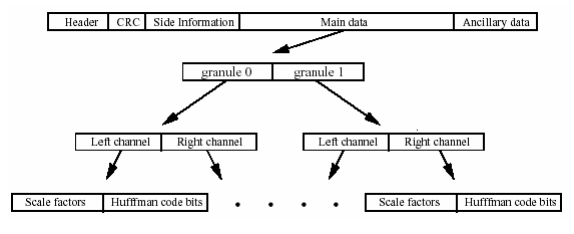
\includegraphics[scale=1]{main_data_layout.png}
				\caption{Struttura del campo Main Data in modalità stereo.}
				\label{fig:main_data_layout}
			\end{figure}
			
			\begin{itemize}
				\item \textit{Fattori di scala}: i \textit{fattori di scala} (o \textit{scalefactor}) vengono utilizzati per ridurre il rumore da quantizzazione e rappresentano delle approssimazioni delle bande critiche dell'orecchio umano (che sono 24). Se scelti correttamente in fase di codifica, la maggior parte del rumore di quantizzazione sparirà, per effetto del mascheramento. Per ogni banda di fattori di scala, viene trasmesso (scelto) un solo fattore di scala. Il campo scfsi determina se (e quali) fattori di scala sono condivisi dai due granuli, in modo da trasmetterli una sola volta. I bit effettivi allocati per i fattori di scala dipendono dal valore del campo scalefac\_compress.\\
					La suddivisione delle frequenze dello spettro in bande di fattori di scala è fissata a seconda del tipo di finestra e della sampling frequency. La suddivisione effettiva è memorizzata in tabelle all'interno dell'encoder e del decoder MP3.
				
				\item \textit{Codifica Huffman}: questa parte dei dati principali contiene i valori codificati tramite codifica di Huffman. Le informazioni su come decodificare questi dati sono contenute nel campo Side Information. Ricordiamo che i valori delle regioni big values sono codificati a coppie, mentre quelli della regione count1 sono codificati a gruppi di 4.
				
			\end{itemize}
		
		\subsection{Ancillary Data} \label{subsec:ancillary_data}
			
			La parte di dati aggiuntivi è opzionale e la sua lunghezza è variabile e non esplicitata. Inizia subito dopo la codifica Huffman del secondo granulo ed arriva fino alla word di sincronizzazione del frame successivo. Questi dati possono essere usati per scopi specifici all'interno di determinate applicazioni.
		
	\section{ID3} \label{sec:id3}
		
		Anche se l'MP3 riesce ad ottenere una notevole compressione audio senza un'eccessiva perdita di qualità, esso manca della possibilità di aggiungere informazioni testuali. Infatti, specialmente per quando riguarda le canzoni, risulta molto comodo salvare all'interno del file \texttt{.mp3}  informazioni testuali come autore o titolo della canzone.\\
		Per soddisfare queste esigenze nacque il cosiddetto ID3, ovvero una serie di tag (di 128 byte) memorizzati alla fine del file \texttt{.mp3}. I tag disponibili erano i seguenti:
		
		\begin{itemize}
			\item titolo (30 byte);
			\item artista (30 byte);
			\item album (30 byte);
			\item anno (4 byte);
			\item commento (30 byte);
			\item genere (1 byte).
		\end{itemize}
		
		Inoltre un file \texttt{.mp3} che volesse fare uso dei tag ID3 doveva scrivere subito dopo i dati aggiuntivi la parola ``TAG'', per indicare dove iniziavano i tag ID3. Escludendo la parola ``TAG'', la somma dei tag ID3 misurava sempre 128 byte (lo spazio inutilizzato veniva riempito con zeri).\\
		\\
		In una variante dell'ID3, detta ID3 v1.1 (Figura \ref{fig:id3v1_1_layout}) al tag del commento sono stati sottratti due bit per aggiungere un tag \textit{traccia} (riferendosi al numero di traccia della canzone nel CD di provenienza) di 1 byte ed un byte nullo tra il commento ed il numero di traccia.\\
		
		\begin{figure}[h!]
			\centering
				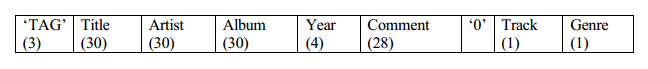
\includegraphics[scale=1]{id3v1_1_layout.png}
			\caption{Struttura dei tag ID3 v1.1.}
			\label{fig:id3v1_1_layout}
		\end{figure}
		
		Le prime versioni di ID3, tuttavia, avevano diversi aspetti negativi, come il fatto di avere pochi campi e che questi avessero una lunghezza massima di 30 byte. Inoltre, dato che le informazioni erano memorizzate alla fine del file \texttt{.mp3} non era possibile ottenerle durante uno streaming in tempo reale. Venne quindi rilasciata una versione più complessa, detta ID3 v2, che memorizzava i tag all'inizio del file \texttt{.mp3}, metteva a disposizione più campi e non imponeva un limite massimo di byte, in quanto supportava dimensioni dinamiche. Attualmente (\monthyear\today) l'ultima versione rilasciata dell'ID3 è l'ID3 v2.4.